Comme expliqué plusieurs fois précédemment, assurer la scalabilité de l'application est un point crucial de ce travail de Bachelor. En effet, l'application doit tenir la charge d'un nombre de festivaliers potentiellement important en simultané.

\section{Tests de montée en charge}

Afin de simuler un nombre important de festivaliers, il est nécessaire de mettre en place un outil permettant de reproduire de réels utilisateurs. Dans la plupart des cas, ce type de test se contente de réaliser un nombre conséquent de requêtes HTTP sur l'application afin de vérifier diverses métriques. Dans le cas de \gls{beeplace}, il ne s'agirait pas d'une solution très intéressante. En effet, l'obstacle majeur à la scalabilité de l'application est la communication WebSocket, qui s'occupe de toute la synchronisation des données entre les utilisateurs. Aucun appel HTTP n'est réalisé par le client vers le serveur, toute l'information transite par WebSocket. Aussi bien l'état initial du canvas que la pose d'un pixel ou encore la réception des pixels des autres utilisateurs. Il faut donc avoir cet aspect bien à l'esprit lors du choix de l'outil de test.

\subsection{Déploiement de l'application}

Afin de tester les limites de l'application sans affecter la version en production, elle est déployée sur une seconde machine virtuelle à l'adresse suivante \href{https://dev-place.beescreens.ch}{dev-place.beescreens.ch}. Les spécifications de cette machine virtuelle sont les suivantes:

\begin{itemize}
  \item CPU 4 c\oe{}urs Intel(R) Xeon(R) CPU E5-2697 v4 @ 2.30GHz
  \item 4 Go de RAM
  \item 50 Go de disque
\end{itemize}

Ces spécifications sont quasiment identiques à celles de la machine virtuelle utilisée pour la version en production. La version en production dispose de 8 Go de RAM au lieu de 4 Go. Grâce à cela, il est possible de tester l'application dans des conditions similaires à la version en production.

\gls{beeplace} est déployée sur cette machine virtuelle à l'aide de Docker et de Docker Compose. La configuration utilisée est la même que pour la version en production. Celle-ci est disponible dans le répertoire \texttt{deployment/beeplace} du répertoire Git.

\subsection{Choix de l'outil}

Pour pouvoir tester la communication WebSocket, il faut tester l'implémentation choisie, à savoir Socket.IO. En effet, Socket.IO utilise son propre protocole de communication~\cite{socket-io-protocol} au-dessus des WebSockets classiques, qui n'est pas forcément supporté par tous les outils de test. La documentation officielle de Socket.IO propose deux manières~\cite{socket-io-load-testing} de tester une application utilisant Socket.IO:

\begin{enumerate}
  \item Utiliser l'outil Artillery~\cite{artillery}
  \item Créer un nombre important de clients Socket.IO manuellement
\end{enumerate}

La deuxième solution n'est pas l'idéale car elle ne permet pas d'avoir des statistiques très poussées sur les performances de l'application. En effet, il est compliqué de récupérer un nombre suffisant de métriques sans finir par développer son propre outil de test. Afin de ne pas réinventer la roue, le choix initial s'est porté sur Artillery.

\subsubsection{Artillery}

Artillery propose différents moteurs utilisables pour tester une application. Il existe donc un moteur Socket.IO permettant d'avoir une solution clé en main pour tester facilement \gls{beeplace}. Les tests sont définis dans un fichier de configuration YAML, qui permet de définir les différentes phases de test ainsi que le comportement des utilisateurs virtuels (appelés scénarios). Ce fichier YAML peut importer un fichier JavaScript afin d'ajouter de la logique supplémentaire aux tests.

\begin{listing}[h]
  \inputminted[linenos]{yaml}{assets/figures/artillery-test.yml}
  \caption{Test de montée en charge avec Artillery}
  \label{listing:artillery}
\end{listing}

Le test d'exemple \ref{listing:artillery} génère 1000 utilisateurs en une minute (soit environ 16 à 17 utilisateurs par seconde). Chaque utilisateur va dessiner trois pixels aléatoirement sur le canvas et attendre ensuite 30 secondes. Cette attente est importante car le client va recevoir les pixels des autres utilisateurs pendant cette période, ce qui simule un comportement plus réaliste. La logique pour générer un pixel aléatoire ainsi que la fingerprint sont définis dans le fichier JavaScript importé \texttt{functions.js}.

Cette solution très simple à mettre en place semble idéale. Cependant, un nombre important de problèmes est survenu:

\begin{itemize}
  \item Le script lance parfois une erreur \texttt{Error: Callback was already called.} qui stoppe l'exécution du test. Plusieurs personnes semblent avoir le même problème sur \gls{github}~\cite{artillery-callback-issue} mais aucune solution n'a encore été trouvée. Utiliser un outil qui n'est pas stable n'est pas envisageable.
  \item Artillery ne permet pas de tester facilement la communication du serveur vers les clients. En effet, l'outil est plus adapté à la communication client-serveur, ce qui est problématique afin de récupérer par exemple la configuration du canvas ou encore les pixels des autres utilisateurs.
  \item Artillery ne met pas à disposition des métriques très utiles dans ses résultats concernant les WebSockets ou Socket.IO. En effet, il n'est pas possible de récupérer la latence de la connexion WebSocket, qui est l'indicateur le plus important dans le cas de \gls{beeplace}. Artillery met à disposition une métrique \texttt{socketio.response\_time} qui pourrait être intéressante mais malheureusement celle-ci ne dépasse pas les quatre millisecondes, même lorsque l'application n'arrive plus à répondre, ce qui est très peu réaliste.
\end{itemize}

Ces raisons ont poussé à abandonner Artillery et à chercher une autre solution. Le code source des recherches effectuées avec Artillery n'est plus disponible dans le répertoire \gls{beescreens} mais reste accessible via un commit spécifique \footnote{Voir commit no. \href{https://gitlab.com/beescreens/beescreens/-/merge_requests/255/diffs?commit_id=98e5e73eae3f9ed77026245cc727aa42728cac3b}{98e5e73eae3f9ed77026245cc727aa42728cac3b}}.

\subsubsection{k6}

k6~\cite{k6} est un outil de test de performance open-source écrit en Go. Il fait partie des outils de test de montée en charge les plus populaires avec plus de 20'000 stars sur \gls{github} et est utilisé par de nombreuses entreprises comme Amazon, Microsoft ou encore \gls{gitlab}. Son avantage principal dans le cas de \gls{beeplace} est que les tests s'écrivent en JavaScript (ou en TypeScript), ce qui permet encore une fois de garder une base de code commune avec le reste des applications.

k6 gère les WebSockets grâce au module expérimental \texttt{k6/experimental/websockets}~\cite{k6-websockets}. Celui-ci implémente l'API WebSocket du navigateur, ce qui permet d'écrire le même code qu'habituellement. Cependant, comme évoqué précédemment, Socket.IO utilise son propre protocole au-dessus des WebSockets, ce qui n'est pas pris en charge nativement par le module k6~\cite{k6-socket-io-issue}. Heureusement, un développeur a mis à disposition sur \gls{github} une implémentation de Socket.IO pour k6~\cite{k6-socket-io}. Celle-ci propose une classe \texttt{K6SocketIO} permettant d'interagir bien plus facilement avec notre serveur Socket.IO.

Cette implémentation initiale n'est pas la plus aisée mais une fois mise en place, l'écriture des tests est assez concise et k6 met à disposition de nombreuses métriques lors des résultats des tests. La plus intéressante dans le cas de \gls{beeplace} est la latence de la connexion WebSocket comme discuté précédemment. Celle-ci est disponible via la métrique \texttt{ws\_connecting} de k6. Il est possible de vérifier que la valeur de cette métrique ne dépasse pas un certain seuil en utilisant la configuration présentée dans le listing \ref{listing:k6-thresholds}.

\begin{listing}[H]
  \begin{minted}[breaklines, linenos]{js}
  thresholds: {
    ws_connecting: [{ threshold: 'p(95)<1200', abortOnFail: true }],
  }
\end{minted}
  \caption{Utilisation de la latence de la connexion WebSocket dans k6}
  \label{listing:k6-thresholds}
\end{listing}

Cet exemple de configuration permet de vérifier que 95\% des connexions WebSocket ne dépassent pas 1200 millisecondes. Si ce seuil est dépassé, le test est considéré comme un échec et s'arrête. Ces chiffres seront discutés plus loin lors de la création du test. Cette fonctionnalité de seuil sera particulièrement utile dans la phase d'optimisation du code \ref{sec:optimisations} afin de vérifier que les changements apportés aient un impact positif sur la latence des connexions.

\subsubsection{Solution choisie}

Le choix s'est porté sur k6. Les raisons principales ont pour la plupart déjà été évoquées mais en voici un petit récapitulatif:

\begin{itemize}
  \item k6 permet une plus grande liberté dans l'écriture des tests grâce à l'utilisation d'un vrai langage de programmation (JavaScript) plutôt que d'un fichier de configuration YAML.
  \item k6 met à disposition dans ses résultats des métriques plus intéressantes pour tester la communication WebSocket.
  \item k6 est plus populaire et il est donc plus facile de trouver la documentation nécessaire pour résoudre les problèmes rencontrés.
\end{itemize}

\subsection{Implémentation du test}

\subsubsection{Types de tests}

Il est tout d'abord nécessaire de trouver quel type de test convient le mieux à la situation. La documentation k6 propose six types de tests de montée en charge:

\begin{figure}[H]
  \centering
  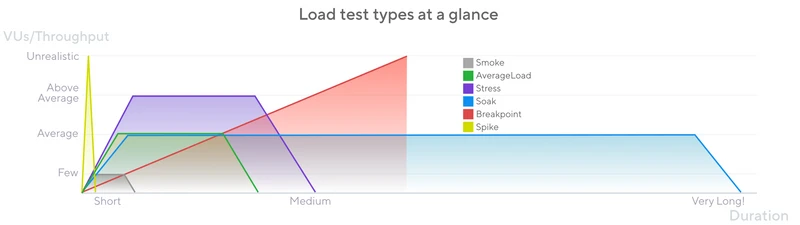
\includegraphics[width=1\textwidth]{./assets/figures/load-test-types.png}
  \begin{center}
    \textit{Schéma issu de la documentation k6~\cite{k6-load-test-types}}
  \end{center}
  \caption{Types de tests de montée en charge}
  \label{fig:load-test-types}
\end{figure}

\begin{itemize}
  \item \textbf{Smoke tests}: permettent de valider que le script de test fonctionne et que le système fonctionne correctement sous une charge minimale.
  \item \textbf{Average-load tests}: évaluent les performances du système dans des conditions normales prévues.
  \item \textbf{Stress tests}: évaluent les performances du système à ses limites, lorsque la charge dépasse la moyenne prévue.
  \item \textbf{Soak tests}: évaluent la fiabilité et les performances du système sur des périodes prolongées.
  \item  \textbf{Spike tests}: valident le comportement et la survie du système en cas d'augmentation soudaine, brève et massive de l'activité.
  \item \textbf{Breakpoint tests}: augmentent progressivement la charge afin d'identifier les limites de capacité du système.
\end{itemize}

Le type le plus utile dans l'état actuel de \gls{beeplace} est le \textbf{Breakpoint test}. En effet, ce type de test permet d'observer facilement si les optimisations réalisées sont efficaces. Plus la charge supportée avant que le système ne s'effondre est élevée, plus les optimisations sont utiles.

\subsubsection{Architecture}

Le code est séparé en deux parties: le code générique permettant de rendre compatible k6 avec Socket.IO et le test en lui-même. Le code générique est placé dans un package nommé \texttt{@beescreens/benchmarks} et est importé dans le test \texttt{apps/beeplace/tests/load-tests}. Ce code pourrait, dans le futur, être utilisé pour tester d'autres applications du projet \gls{beescreens} implémentant également Socket.IO, comme Pimp My Wall par exemple.

\begin{listing}[H]
  \begin{tcolorbox}[arc=0mm,colback=white!5!white]
    \dirtree{%
      .1 /.
      .2 apps.
      .3 beeplace.
      .4 tests.
      .5 load-tests.
      .4 ....
      .3 ....
      .2 packages.
      .3 benchmarks.
      .3 ....
    }
  \end{tcolorbox}
  \caption{Structure des tests de montée en charge de \gls{beeplace}
    \label{listing:load-tests-structure}}
\end{listing}

\subsubsection{Test avec k6}

Le test utilisé est une Breakpoint test, l'implémentation a été séparée en trois parties afin de pouvoir la commenter plus facilement.

\begin{listing}[H]
  \inputminted[linenos]{ts}{assets/figures/breakpoint-test-1.ts}
  \caption{Breakpoint test avec k6 - Fonction principale}
  \label{listing:k6-breakpoint-test-1}
\end{listing}

La fonction principale du listing \ref{listing:k6-breakpoint-test-1} est exécutée pour chaque utilisateur virtuel. Elle se connecte à l'endpoint WebSocket grâce à la classe \texttt{K6SocketIo} du package précédemment évoqué \texttt{\\@beescreens/benchmarks}. Elle appelle ensuite la fonction \texttt{drawMaxRandomPixels} détaillée dans le listing \ref{listing:k6-breakpoint-test-3} qui contient le comportement propre à l'utilisateur. Les erreurs sont également comptabilisées afin de les afficher à la fin du test.

\begin{listing}[H]
  \inputminted[linenos]{ts}{assets/figures/breakpoint-test-2.ts}
  \caption{Breakpoint test avec k6 - Options}
  \label{listing:k6-breakpoint-test-2}
\end{listing}

Le listing \ref{listing:k6-breakpoint-test-2} présente les options du test. Le test dure un maximum de 5 minutes et va ajouter un nombre d'utilisateurs virtuels croissant jusqu'à l'objectif souhaité de 1000 utilisateurs. Le test ne se soucie pas de l'éventuelle latence de l'application grâce à l'exécuteur \texttt{ramping-arrival-rate}.

Le \texttt{threshold} défini permet d'arrêter le test lorsque le temps de chargement est jugé trop conséquent pour une utilisation fluide de l'application. Dans cet exemple, le test s'arrête si le temps de connexion WebSocket dépasse \textbf{1200 millisecondes} pour \textbf{95\%} des utilisateurs virtuels.

Ces nombres sont choisis de la manière suivante: plusieurs valeurs sont mises à disposition par k6 pour les différentes métriques des résultats: \texttt{avg}, \texttt{med}, \texttt{min}, \texttt{max}, \texttt{p(90)} et \texttt{p(95)}. Ces valeurs correspondent respectivement à la moyenne, la médiane, la valeur minimale, la valeur maximale, la valeur du percentile 90 et la valeur du percentile 95. Le percentile 95 indique par exemple la valeur pour laquelle 95\% des utilisateurs virtuels se trouvent en dessous. Utiliser le percentile 95 permet de ne pas prendre en compte les valeurs extrêmes qui pourraient être dues à des problèmes de réseau par exemple, tout en ayant une valeur représentative de la majorité des utilisateurs virtuels.

Concernant la valeur choisie pour la latence de la connexion WebSocket, elle se base sur les bonnes pratiques du web. Un article~\cite{how-fast-should-a-website-load-in-2023} indique que le chargement d'un site, d'autant plus sur mobile, devrait idéalement se faire en une à deux secondes. La valeur de 1200 millisecondes est donc choisie pour être dans la partie basse de cette intervalle afin d'avoir une certaine marge. En effet, il faut également prendre en compte que la latence est calculée uniquement sur la connexion WebSocket avec le backend. Pour un utilisateur réel, il faudrait également ajouter le délai du chargement du frontend de l'application.

\begin{listing}[H]
  \inputminted[linenos]{ts}{assets/figures/breakpoint-test-3.ts}
  \caption{Breakpoint test avec k6 - Comportement des utilisateurs virtuels}
  \label{listing:k6-breakpoint-test-3}
\end{listing}

Finalement, le listing \ref{listing:k6-breakpoint-test-3} présente le comportement des utilisateurs virtuels. Chaque utilisateur virtuel fait une requête sur le frontend de l'application afin de simuler plus authentiquement un utilisateur réel en ajoutant une charge sur le frontend. Il se connecte ensuite à l'endpoint WebSocket et récupère le canvas actuel ainsi que les options de configuration. Il pose ensuite le nombre de pixels maximum (3 dans cet exemple) sur le canvas de manière aléatoire. Pour finir, il attend 30 secondes avant de se déconnecter afin de simuler la réception des pixels dessinés par les autres utilisateurs. Le nombre de pixels dessinés est comptabilisé afin de l'afficher dans les résultats du test.

Poser des pixels de position et de couleur aléatoires permet d'obtenir de jolis résultats visuellement comme affiché sur la figure \ref{fig:load-test-result}.

\begin{figure}[H]
  \centering
  
\includegraphics[width=0.6\textwidth]{assets/figures/load-test-result.png}
  \caption{Résultat visuel des tests de montée en charge}
  \label{fig:load-test-result}
\end{figure}

\subsection{Résultats initiaux}

Les résultats des tests k6 contiennent de nombreuses métriques intéressantes. Les comparaisons vont se baser sur un échantillon d'entre elles mais un exemple complet est disponible avec le lien en note de bas de page \footnote{\url{https://github.com/heig-vkaelin/template-tb/blob/main/assets/external/k6-result.txt}}.

Les métriques utilisées pour pouvoir vérifier par la suite si les optimisations sont efficaces sont les suivantes:

\begin{itemize}
  \item Temps d'exécution du test avant que le seuil de latence ne soit atteint (1200 ms pour la connexion WebSocket).
  \item Nombre d'utilisateurs virtuels créés
  \item Nombre de pixels dessinés
\end{itemize}

Le test a été lancé 10 fois afin de prévenir les éventuelles erreurs de mesure. Les résultats sont présentés dans le tableau \ref{table:k6-initial-results}.

\begin{table}[H]
  \centering
  \begin{tabular}{|l|l|l|l|}
    \hline
    \textbf{Test}    & \textbf{Temps d'exécution} & \textbf{Utilisateurs virtuels} & \textbf{Pixels dessinés} \\ \hline
    1                & 22385.053 ms               & 703                            & 1317                     \\ \hline
    2                & 20921.705 ms               & 589                            & 1168                     \\ \hline
    3                & 22353.215 ms               & 704                            & 1366                     \\ \hline
    4                & 23175.281 ms               & 707                            & 1389                     \\ \hline
    5                & 30976.405 ms               & 797                            & 1672                     \\ \hline
    6                & 24097.739 ms               & 702                            & 1382                     \\ \hline
    7                & 25074.294 ms               & 699                            & 1319                     \\ \hline
    8                & 22141.945 ms               & 630                            & 1455                     \\ \hline
    9                & 32062.651 ms               & 786                            & 1596                     \\ \hline
    10               & 20743.08 ms                & 452                            & 1056                     \\ \hline
    \textbf{Moyenne} & \textbf{24393.147 ms}      & \textbf{676.9}                 & \textbf{1372}            \\ \hline
    \textbf{Médiane} & \textbf{22780.167 ms}      & \textbf{702.5}                 & \textbf{1374}            \\ \hline
  \end{tabular}
  \caption{Résultats initiaux des tests de montée en charge avec k6}
  \label{table:k6-initial-results}
\end{table}

La médiane sera préférée à la moyenne pour les futures comparaisons car elle est moins sensible aux valeurs extrêmes. Même si les valeurs des 10 itérations du test sont relativement proches dans ce cas-ci.

Pour conclure, avec la version initiale de \gls{beeplace}, le test est exécuté pendant environ \textbf{23 secondes} en créant \textbf{702 utilisateurs virtuels} qui dessinent au total \textbf{1374 pixels}.

\section{Profiling}

Pour trouver plus facilement les optimisations à effectuer, il est nécessaire de profiler l'application. Le profiling permet de trouver les parties du code qui prennent le plus de temps à s'exécuter et qui sont donc plus intéressantes à optimiser.

\subsection{Choix de l'outil}

\subsubsection{Solution native à Node.js}

Node.js propose un outil de profiling natif qu'il est possible d'appeler en utilisant simplement l'argument \texttt{node -{}-prof}. Cet outil permet de générer un fichier de profiling illisible en lui-même. Heureusement, l'argument \texttt{node -{}-prof-process} permet d'analyser ce fichier de log et de générer un fichier textuel plus compréhensible.

L'inconvénient de cette approche réside dans le fait que le fichier texte des résultats reste peu pratique à utiliser. Il est difficile de voir quelles fonctions sont les plus gourmandes en ressources sans une interface graphique avec un système de filtre.

\subsubsection{Parca}

Parca~\cite{parca} est un outil de profiling open-source développé par l'équipe derrière le projet Kubernetes. Son objectif est d'être très léger afin de pouvoir être utilisé en production sans affecter les performances de l'application. Ces performances sont possibles car Parca utilise une approche basée sur la technologie eBPF (extended Berkeley Packet Filter)~\cite{ebpf}. Cette technique permet d'exécuter du code dans le noyau Linux sans avoir besoin de modifier directement le code source.

Le problème de cette technique est qu'elle n'est pas supportée par tous les systèmes d'exploitation. Parca ne peut donc pas être utilisé sur Windows ou macOS. Il n'est donc pas possible de tester en local l'optimisation avec Parca dans le cadre du projet \gls{beeplace}. Cependant, Parca reste un choix intéressant lorsqu'il s'agira de tester l'optimisation sur le serveur de production.

\subsubsection{Pyroscope}

Pyroscope~\cite{pyroscope} est un outil de profiling également open-source développé par l'équipe Grafana Labs. Il s'agit de la même équipe qui est à l'origine de l'outil de tests de montée en charge k6 que \gls{beeplace} utilise. Pyroscope est utilisable facilement en local avec Docker et propose une intégration avec de nombreux langages de programmation, dont Node.js. Il suffit d'ajouter la dépendance et de lancer le profiling dans le code de l'application. Le code enverra par la suite les données de profiling au serveur Pyroscope toutes les dix secondes.

Malheureusement, le dashboard proposé n'est pas le plus intuitif, il ne met pas à disposition de nombreux filtres et cela rend l'analyse des résultats difficile.

\subsection{Clinic.js}

Clinic.js~\cite{clinicjs} est une suite d'outils de profiling développé par des membres de l'équipe derrière Node.js. Il suffit d'installer le projet comme une dépendance \gls{npm} globale pour avoir accès à quatre outils différents:

\begin{itemize}
  \item \textbf{Doctor} permet de diagnostiquer les problèmes de performance d'une applications en identifiant les symptômes tels que des problèmes de lecture/écriture ou des problèmes de mémoire.
  \item \textbf{Flame} permet d'identifier rapidement et précisément les goulots d'étranglement du code grâce à des graphiques en flammes qui visualisent les chemins d'exécution les plus fréquents.
  \item \textbf{Bubbleprof} observe les opérations asynchrones de l'application et les affiche dans un graphique en bulles pour visualiser les différents délais.
  \item \textbf{Heap Profiler} met également à disposition des graphiques en flammes comme le mode Flame mais pour l'utilisation de la mémoire.
\end{itemize}

Le mode le plus intéressant pour le projet \gls{beeplace} est le mode Flame. Il permet de visualiser les chemins d'exécution les plus fréquents et donc de trouver les fonctions qui prennent le plus de temps à s'exécuter. Celles-ci doivent donc être optimisées en priorité.

Clinic.js est plus pensée pour être utilisé localement. En effet, le rapport de profiling est généré lorsque l'application Node s'arrête. Ce qui n'est pas envisageable en production. Il est donc nécessaire de tester l'optimisation en local avant de la déployer sur le serveur de production.

\subsection{Solution choisie}

Le choix final s'est donc tourné vers un profiling en local à l'aide de Clinic.js afin d'avoir un retour rapide sur l'efficacité des optimisations réalisées. Pour récapituler, le processus est le suivant:

\begin{enumerate}
  \item Lancer l'application Node.js en local avec Clinic.js: \texttt{clinic flame -{}- node app.js}
  \item Démarrer le test de montée en charge en local avec k6
  \item Arrêter l'application Node.js une fois le test terminé
  \item Analyser le rapport de Clinic.js
  \item Optimiser le code
  \item Recommencer
\end{enumerate}

Une fois les optimisations effectuées et testées en local, il est possible de les déployer sur le serveur de test de montée en charge pour comparer les résultats avec la version initiale \ref{table:k6-initial-results}.

\subsection{Analyses}

\subsubsection{Rapport initial}

% Used results: file:///Users/valentin/code/beescreens/apps/beeplace/backend/.clinic/59944.clinic-flame.html

\begin{figure}[H]
  \centering
  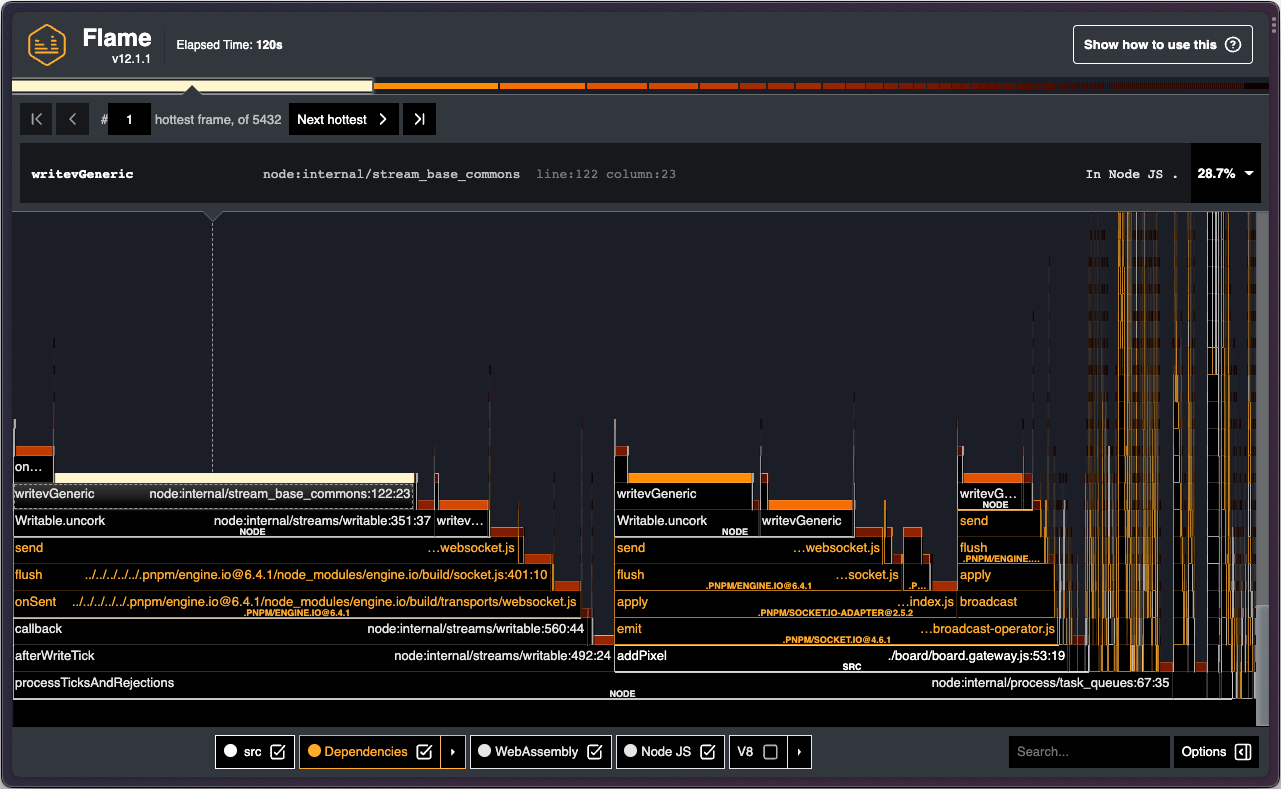
\includegraphics[width=1\textwidth]{./assets/figures/flame/flame1-overview.png}
  \caption{Vision d'ensemble du rapport initial de Clinic.js}
  \label{fig:flame1-overview}
\end{figure}

A la fin du test de montée en charge, l'analyse réalisée par Clinic.js avec son graphique en flammes visible sur la figure \ref{fig:flame1-overview} n'est pas facilement interprétable. En effet, initialement les fonctions ne sont pas filtrées. Le graphique affiche donc les fonctions venant du code Node.js ainsi que des dépendances en plus du code propre au projet. Il est tout de même possible de voir que la plupart des fonctions affichées concernent l'écriture de données dans le cadre des WebSockets avec des fonctions comme \texttt{writevGeneric}, \texttt{onwrite} ou \texttt{flush}.

En filtrant pour garder uniquement le code du projet, car c'est celui-ci qu'il est possible d'optimiser, le graphique devient plus lisible comme le montre la figure \ref{fig:flame1-filtered}.

\subsubsection{Rapport filtré}

\begin{figure}[H]
  \centering
  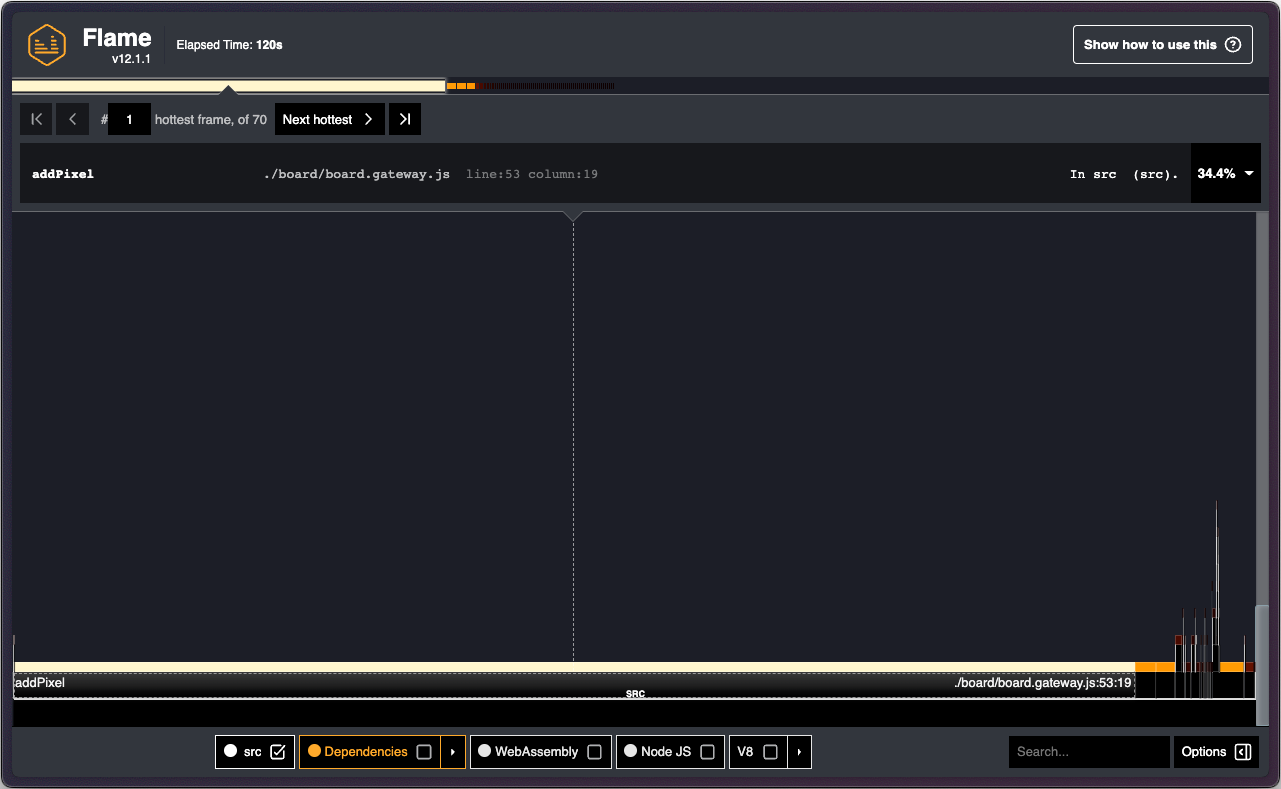
\includegraphics[width=1\textwidth]{./assets/figures/flame/flame1-filtered.png}
  \caption{Vision filtrée du rapport initial de Clinic.js}
  \label{fig:flame1-filtered}
\end{figure}

Plus de 34\% du temps d'exécution est passé dans la fonction \texttt{addPixel}. Celle-ci est appelée à chaque fois qu'un utilisateur envoie un nouveau pixel au serveur. Elle contient la logique suivante:

\begin{enumerate}
  \item Récupérer le nombre de pixels posés par l'utilisateur
  \item Ajouter le pixel dans le BitField Redis ainsi que dans l'historique PostgreSQL
  \item Incrémenter le nombre de pixels posés par l'utilisateur (ou le créer s'il n'existe pas)
  \item Partager le pixel avec les autres utilisateurs connectés (broadcast WebSockets)
\end{enumerate}

La deuxième fonction la plus utilisée est \texttt{placePixel} avec 0.7\% du temps d'exécution. Celle-ci s'occupe du point numéro 2. de la fonction \texttt{addPixel}. Elle est donc fortement liée à la fonction \texttt{addPixel}.

Les fonctions suivantes ne dépassent pas les 0.6\% du temps d'exécution, il s'agit notamment de la récupération de l'état actuel du BitField Redis ainsi que de l'initialisation de la connexion WebSockets.

Il faudra donc dans un premier temps se concentrer sur la fonction \texttt{addPixel}. Pour commencer, il est possible de regrouper les tâches de la fonction en deux catégories à optimiser:

\begin{enumerate}
  \item Sauvegarde du pixel
  \item Broadcast du pixel
\end{enumerate}

Afin de vérifier quelle partie doit être optimisée en priorité, il est possible de se concentrer sur la fonction \texttt{addPixel} et d'afficher à nouveau les fonctions des dépendances comme le montre la figure \ref{fig:flame1-addPixel}.

\subsubsection{Fonction addPixel}

\begin{figure}[H]
  \centering
  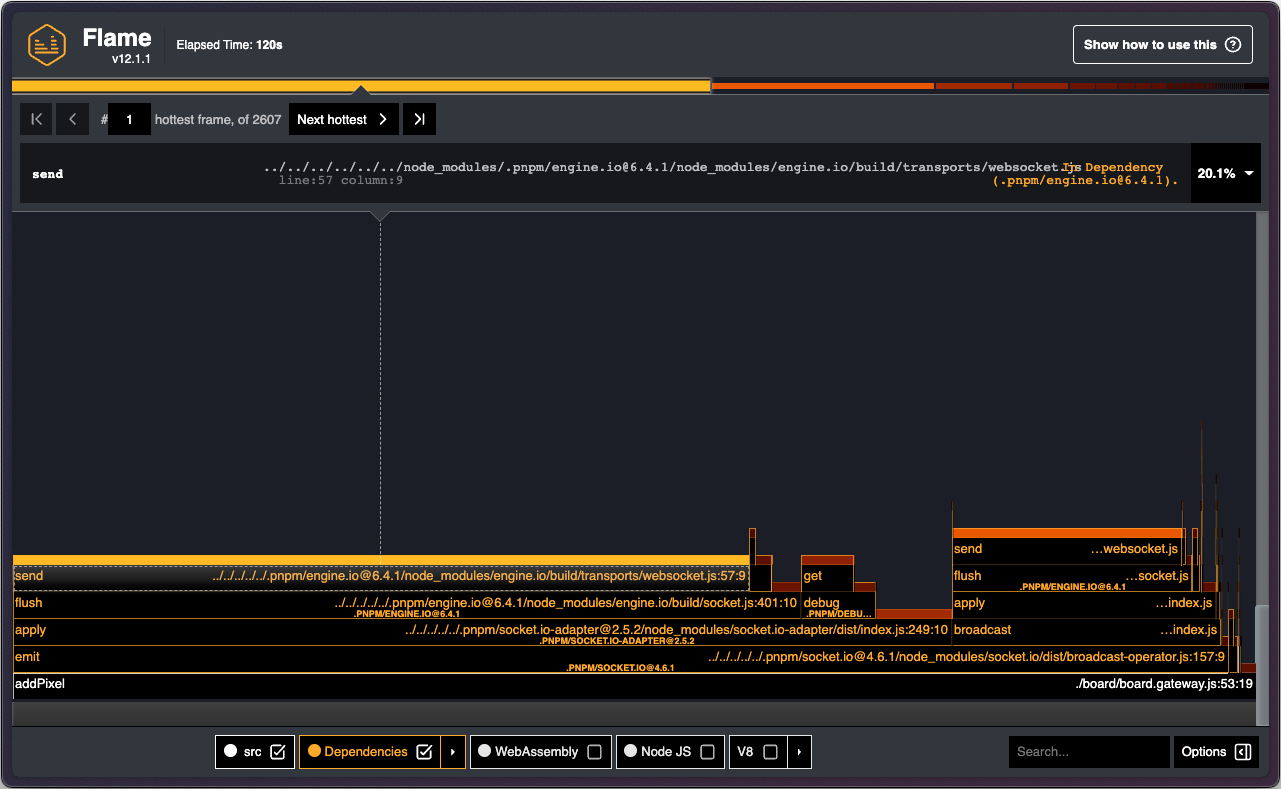
\includegraphics[width=1\textwidth]{./assets/figures/flame/flame1-addPixel.png}
  \caption{Zoom sur la fonction \texttt{addPixel} du rapport initial de Clinic.js}
  \label{fig:flame1-addPixel}
\end{figure}

Cette figure \ref{fig:flame1-addPixel} qui se concentre sur la fonction \texttt{addPixel} montre rapidement qu'une grande majorité du temps d'exécution de la fonction concerne le broadcast du pixel avec Socket.IO. En effet, la fonction \texttt{send} de Socket.IO représente 26.5\% du temps d'exécution de la fonction \texttt{addPixel} (20.1\% + 6.4\%). Concernant la sauvegarde du pixel, le temps d'exécution de la fonction \texttt{placePixel} est si faible qu'il est affiché comme valant 0\% du temps d'exécution de la fonction \texttt{addPixel}.

\subsubsection{Conclusion initiale}

La fonction \texttt{addPixel}, appelée à chaque fois qu'un utilisateur pose un pixel, est clairement la fonction à optimiser en priorité. Plus précisément, la partie de la fonction qui s'occupe de broadcast le pixel avec Socket.IO à tous les autres utilisateurs connectés.

\section{Optimisations}
\label{sec:optimisations}

\subsection{Mise en place}

Pour comparer facilement les résultats des diverses optimisations, des images \gls{docker} du frontend ainsi que du backend de \gls{beeplace} sont créées avec un tag associé à l'optimisation souhaitée \footnote{\url{https://gitlab.com/beescreens/beescreens/container_registry/4113549}}. Ceci permet de pouvoir facilement changer la version de l'application qui tourne sur la machine virtuelle de test en modifiant simplement le tag de l'image dans les variables d'environnement du fichier \texttt{.env} utilisé lors du déploiement.

Cette mise en place évite d'avoir un laps de temps conséquent entre l'exécution des tests sur les différentes versions. Ceci permet de limiter l'incidence de facteurs externes sur les résultats obtenus.

\subsection{Optimisation du broadcast}

Afin d'optimiser la fonction \texttt{addPixel} vue précédemment, il est possible de revoir la manière d'envoyer le pixel aux autres utilisateurs connectés.

Pour l'instant, le pixel dessiné par l'utilisateur est transmis immédiatement à tous les autres utilisateurs connectés par le serveur. Ce qui engendre un nombre de messages WebSockets envoyés très important. L'idée d'optimisation est de regrouper les pixels dessinés par l'utilisateur dans un intervalle de temps donné et de les envoyer en un seul message WebSockets.

\subsubsection{Implémentation}

Toute la logique est implémentée dans la classe \texttt{BoardGateway}, qui s'occupe de la communication WebSocket.

\begin{listing}[H]
  \inputminted[highlightlines={3,12,18,19,29},linenos]{ts}{assets/figures/opti-interval.ts}
  \caption{Optimisation du broadcast avec un intervalle de temps}
  \label{listing:opti-interval}
\end{listing}

Au démarrage de l'application, un intervalle JavaScript est créé et stocké dans le \texttt{scheduler registry} de Nest afin d'éviter de le stocker directement dans la classe courante. L'intervalle appelle la fonction \texttt{broadcastBoardUpdates} qui s'occupe d'envoyer les pixels dessinés à tous les utilisateurs. Le délai entre chaque rafraîchissement est configurable via la variable d'environnement \texttt{BOARD\_REFRESH\_RATE}. La valeur choisie pour la suite des tests est de 100 millisecondes, comme la version initiale du r/place de \gls{reddit}. Une valeur aussi faible permet d'avoir une expérience utilisateur fluide.

Une Map est utilisée pour stocker les différents pixels dessinés au cours de l'intervalle. Chaque clé de la Map correspond à sa position sur le canvas. Cette implémentation permet de garder uniquement le dernier pixel dessiné à une position donnée. Ainsi, si plusieurs utilisateurs dessinent un pixel à la même position pendant le court intervalle, seul le dernier pixel dessiné sera envoyé aux autres utilisateurs.

Avant d'envoyer la mise à jour aux autres utilisateurs, une vérification est effectuée pour savoir si des pixels ont été dessinés pendant l'intervalle. Si ce n'est pas le cas, l'envoi du message est annulé. Cela permet d'éviter d'envoyer de nombreux messages inutiles aux utilisateurs. Cette vérification permet de se rapprocher du comportement initial de l'application qui envoyait une mise à jour quand un pixel était dessiné. La seule modification potentiellement perceptible est l'ajout des 100 millisecondes de délai.

\subsubsection{Résultats}

Dans la suite des tableaux et des graphiques, la version non optimisée sera notée \textbf{Initiale} et la version optimisée avec l'intervalle sera notée \textbf{Intervalle}.

% DE BASE
% Mean duration: 19197.170700000002 ms
% Median duration: 18908.497000000003 ms

% Mean vusers: 542.3
% Median vusers: 558

% Mean pixels: 1008
% Median pixels: 1017

% INTERVAL
% Mean duration: 30491.0314 ms
% Median duration: 29275.9285 ms

% Mean vusers: 1371.8
% Median vusers: 1348.5

% Mean pixels: 3201.5
% Median pixels: 3078.5

\begin{table}[H]
  \centering
  \begin{tabular}{|l|l|l|l|}
    \hline
    \textbf{Version} & \textbf{Temps d'exécution} & \textbf{Utilisateurs virtuels} & \textbf{Pixels dessinés} \\ \hline
    Initiale         & 18908.497 ms               & 558                            & 1017                     \\ \hline
    Intervalle       & 29275.929 ms               & 1348.5                         & 3078.5                   \\ \hline
  \end{tabular}
  \caption{Médiane des résultats de 10 tests entre le code initial et la première optimisation}
  \label{table:first-opti-results}
\end{table}

\begin{figure}[H]
  \centering
  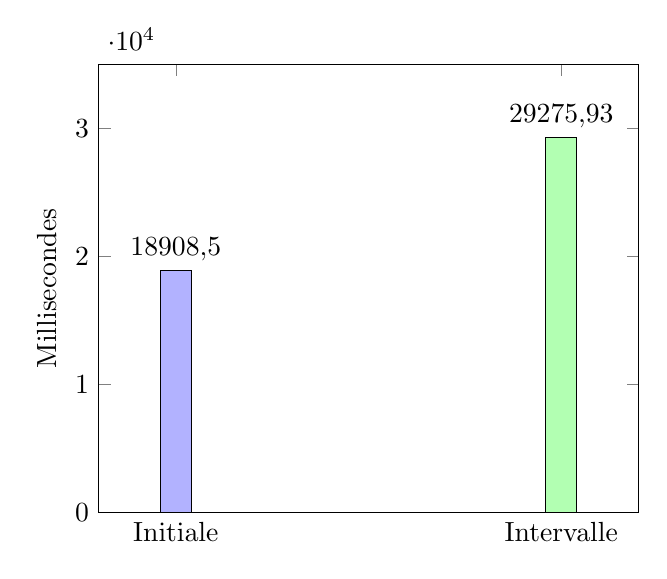
\begin{tikzpicture}
    \begin{axis}[
        /pgf/number format/.cd,
        use comma,
        1000 sep={},
        ylabel={Millisecondes},
        ymin=0,
        ymax=35000,
        xtick={1,2},
        xticklabels={Initiale, Intervalle},
        nodes near coords,
        nodes near coords align={vertical},
        every axis plot/.append style={
            ybar,
            bar width=0.08,
            bar shift=0pt,
            fill
          },
        enlarge x limits={0.2},
      ]
      \addplot[fill=blue!30] coordinates {
          (1,18908.497)
        };
      \addplot[fill=green!30] coordinates {
          (2,29275.929)
        };
    \end{axis}
  \end{tikzpicture}
  \caption{Temps d'exécution du test entre la version initiale et l'optimisation avec l'intervalle}
  \label{fig:chart-opti-initial-interval-duration}
\end{figure}

\begin{figure}[H]
  \centering
  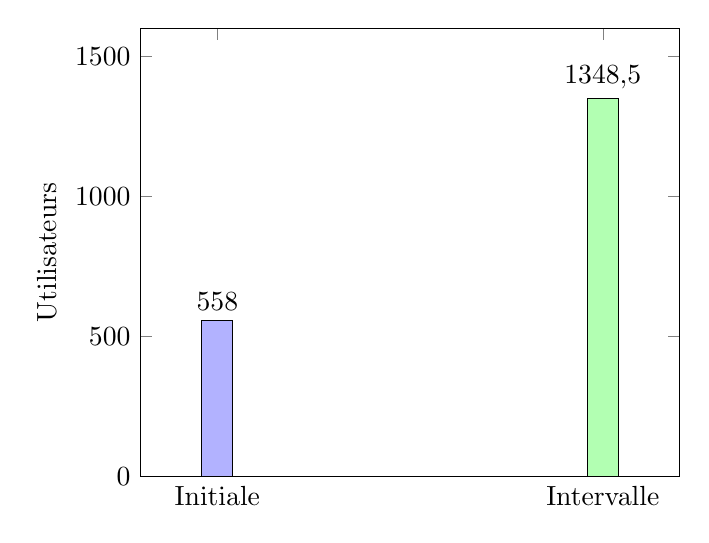
\begin{tikzpicture}
    \begin{axis}[
        /pgf/number format/.cd,
        use comma,
        1000 sep={},
        ylabel={Utilisateurs},
        ymin=0,
        ymax=1600,
        xtick={1,2},
        xticklabels={Initiale, Intervalle},
        nodes near coords,
        nodes near coords align={vertical},
        every axis plot/.append style={
            ybar,
            bar width=0.08,
            bar shift=0pt,
            fill
          },
        enlarge x limits={0.2},
      ]
      \addplot[fill=blue!30] coordinates {
          (1,558)
        };
      \addplot[fill=green!30] coordinates {
          (2,1348.5)
        };
    \end{axis}
  \end{tikzpicture}
  \caption{Utilisateurs supportés entre la version initiale et l'optimisation avec l'intervalle}
  \label{fig:chart-opti-initial-interval-users}
\end{figure}

\begin{figure}[H]
  \centering
  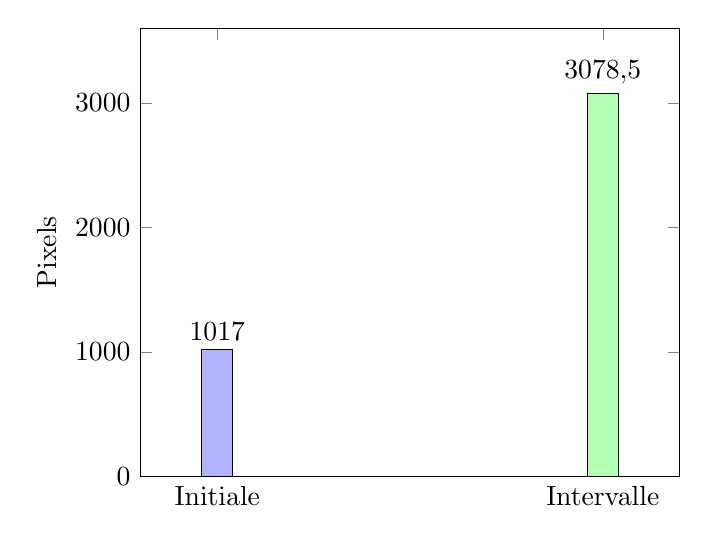
\begin{tikzpicture}
    \begin{axis}[
        /pgf/number format/.cd,
        use comma,
        1000 sep={},
        ylabel={Pixels},
        ymin=0,
        ymax=3600,
        xtick={1,2},
        xticklabels={Initiale, Intervalle},
        nodes near coords,
        nodes near coords align={vertical},
        every axis plot/.append style={
            ybar,
            bar width=0.08,
            bar shift=0pt,
            fill
          },
        enlarge x limits={0.2},
      ]
      \addplot[fill=blue!30] coordinates {
          (1,1017)
        };
      \addplot[fill=green!30] coordinates {
          (2,3078.5)
        };
    \end{axis}
  \end{tikzpicture}
  \caption{Pixels dessinés entre la version initiale et l'optimisation avec l'intervalle}
  \label{fig:chart-opti-initial-interval-pixels}
\end{figure}

Pour conclure, l'optimisation avec l'intervalle est très effective. Cette nouvelle version supporte la montée en charge pendant \textbf{54.82\%} de temps en plus. Le nombre d'utilisateurs virtuels supportés est augmenté de \textbf{141.67\%} et le nombre de pixels dessinés est augmenté de \textbf{202.70\%}.

Le nombre d'utilisateurs supportés avant que le temps de réponse ne devienne trop élevé (plus de 1.2 secondes) est devenu suffisant pour que l'application reste stable même si toutes les personnes présentes lors du Baleinev Festival se connectent en même temps.

Cependant, il est intéressant de vérifier si d'autres optimisations ne pourraient pas être également implémentées et utiles. Un nouveau profiling avec Clinic.js est donc effectué sur cette version.

% Source: file:///Users/valentin/code/beescreens/apps/beeplace/backend/.clinic/51448.clinic-flame.html#selectedNode=5976&zoomedNode=5976&exclude=8000-0-0-6-f000&merged=true

\begin{figure}[H]
  \centering
  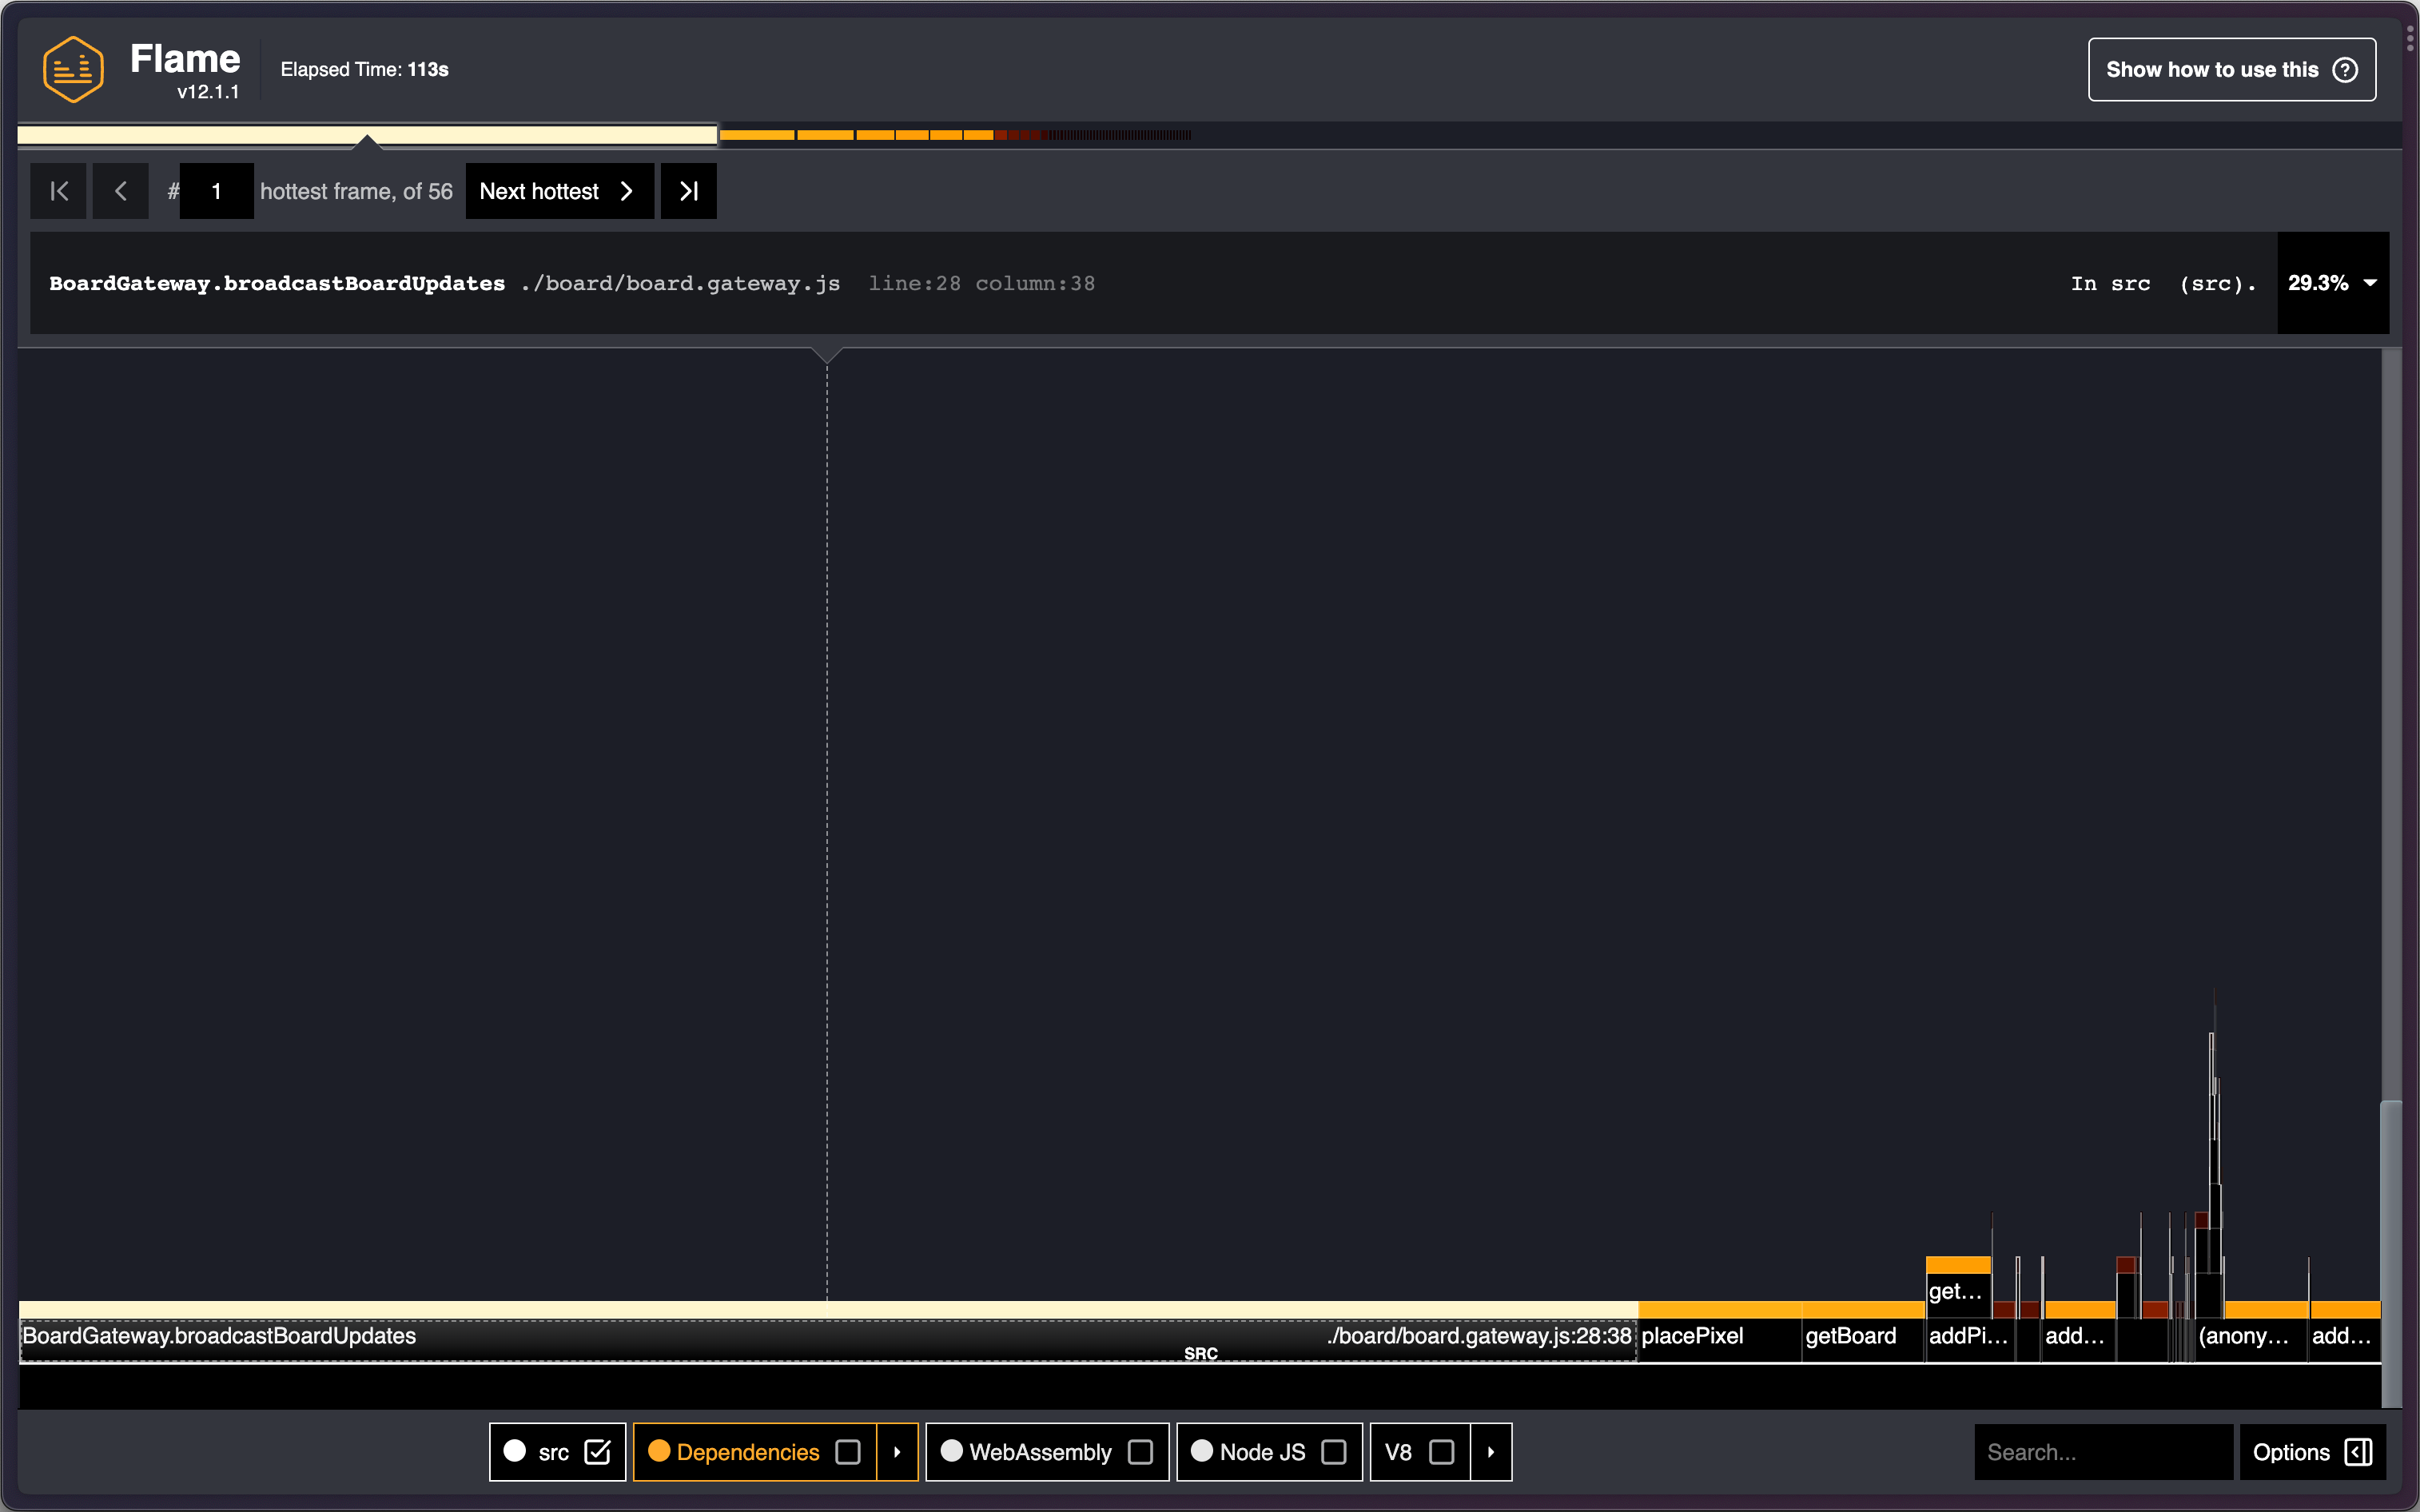
\includegraphics[width=1\textwidth]{./assets/figures/flame/flame2-filtered.png}
  \caption{Vision filtrée du rapport après optimisation avec l'intervalle}
  \label{fig:flame2-filtered}
\end{figure}

En regardant le graphique en flammes de la version optimisée, il est possible de voir que la majorité du temps d'exécution est toujours occupé par la fonction s'occupant uniquement de broadcast les pixels aux utilisateurs, à savoir \texttt{broadcastBoardUpdates}. Il est donc intéressant de rester dans le domaine de l'optimisation de la communication WebSocket par la suite.

\subsection{Format des données}

Actuellement, les pixels sont envoyés sous la forme classique d'un tableau d'objets JSON transformé automatiquement par Socket.IO en chaîne de caractères. Chaque objet contient les coordonnées du pixel ainsi que sa couleur. Les clés sont répétées pour chaque pixel, ce qui augmente la taille du message comme le montre le listing \ref{listing:pixels-initial-json-format}.

\begin{listing}[H]
  \begin{minted}[linenos]{json}
  [
    { "x": 12, "y": 56, "color": 12 },
    { "x": 33, "y": 42, "color": 8 }
    // ...
  ]
\end{minted}
  \caption{Format initial des pixels en JSON}
  \label{listing:pixels-initial-json-format}
\end{listing}

\subsubsection{Format binaire}

La solution la plus optimale pour réduire la taille des messages envoyés consiste à transformer le tableau de pixels dans un format binaire. En effet, chaque pixel est représenté par 3 entiers stockés sur au minimum 2 octets chacun (afin de pouvoir avoir des coordonnées plus grandes que les 255 autorisées sur 1 octet). Un tableau \texttt{Uint16Array} est donc utilisé pour stocker les pixels (16 bits = 2 octets) comme le montre le listing \ref{listing:opti-binary}.

\begin{listing}[H]
  \inputminted[highlightlines={9}, linenos]{ts}{assets/figures/opti-binary.ts}
  \caption{Optimisation du broadcast avec un format binaire}
  \label{listing:opti-binary}
\end{listing}

Du côté du client, il suffit simplement de lire les valeurs trois par trois dans le tableau pour obtenir les pixels individuellement pour les afficher.

Une comparaison rapide de la taille gagnée est réalisable facilement. Les deux pixels précédents sont utilisés comme exemple. Tous les caractères utilisés sont des caractères ASCII, ils utilisent donc 1 octet chacun.

\begin{listing}[H]
  \begin{minted}[linenos]{json}
  [{"x":12,"y":56,"color":12},{"x":33,"y":42,"color":8}] // ->  54 caractères -> 54 octets
  [12,56,12,33,42,8]                     // ->  6 entiers sur 2 octets chacun -> 12 octets
\end{minted}
  \caption{Comparaison entre le format JSON et le format binaire}
  \label{listing:json-vs-binary}
\end{listing}

Le résultat est donc \textbf{4.5 fois} plus léger en utilisant le format binaire. A noter que ce ratio peut être encore meilleur dans le cas où les coordonnées des pixels sont plus grandes. En effet, jusqu'à 65'535, les entiers restent stockés sur 2 octets mais la chaîne de caractère augmente en taille (ex: longueur 5 à partir de 10'000 donc 5 octets).

Pour vérifier si cette optimisation est efficace, un nouveau benchmark est effectué. Les résultats sont présentés dans le tableau \ref{table:second-opti-results}.

\begin{table}[H]
  \centering
  \begin{tabular}{|l|l|l|l|}
    \hline
    \textbf{Version} & \textbf{Temps d'exécution} & \textbf{Utilisateurs virtuels} & \textbf{Pixels dessinés} \\ \hline
    Initiale         & 18908.497 ms               & 558                            & 1017                     \\ \hline
    Intervalle       & 29275.929 ms               & 1348.5                         & 3078.5                   \\ \hline
    Binaire          & 29267.474 ms               & 1332.5                         & 2967                     \\ \hline
  \end{tabular}
  \caption{Médiane des résultats de 10 tests entre trois versions de l'application}
  \label{table:second-opti-results}
\end{table}

Malheureusement, ces résultats ne sont pas très concluants. En effet, la version utilisant du format binaire est légèrement moins performante que la version précédente. Ce comportement peut être expliqué avec le comportement de Socket.IO. Comme l'explique une issue \gls{github}~\cite{socket-io-binary-issue}, Socket.IO envoie deux paquets par message s'il s'agit d'un contenu binaire. Un parseur customisé~\cite{socket-io-msgpack-parser} a été créé par l'équipe de Socket.IO mais il n'a malheureusement pas été possible de le faire fonctionner dans le cadre de \gls{beeplace}. La supposition est que la version de Socket.IO utilisée par NestJS n'est pas compatible avec ce parseur.

\subsubsection{Format string}

Pour ne pas avoir ce souci de deux paquets par message, une seconde tentative d'optimisation est réalisée en utilisant une chaîne de caractère plus optimisée que le format JSON. L'idée est de créer le même tableau que précédemment mais de le transformer en chaîne de caractères en utilisant la fonction \texttt{toString} comme le montre le listing \ref{listing:opti-string}.

\begin{listing}[H]
  \inputminted[highlightlines={5,6}, linenos]{ts}{assets/figures/opti-string.ts}
  \caption{Optimisation du broadcast avec une chaîne de caractères}
  \label{listing:opti-string}
\end{listing}

En prenant toujours les mêmes deux pixels en exemple, le résultat est le suivant:

\begin{listing}[H]
  \begin{minted}[linenos]{json}
  [{"x":12,"y":56,"color":12},{"x":33,"y":42,"color":8}] // ->  54 caractères -> 54 octets
  [12,56,12,33,42,8]                                     // ->  18 caractères -> 18 octets
\end{minted}
  \caption{Comparaison entre le format JSON et le format en chaîne de caractères}
  \label{listing:json-vs-string}
\end{listing}

La version avec la string optimisée est \textbf{3 fois} plus légère que la version initiale en JSON. Il est donc possible de tester cette nouvelle version pour la comparer aux précédentes.

\begin{table}[H]
  \centering
  \begin{tabular}{|l|l|l|l|}
    \hline
    \textbf{Version} & \textbf{Temps d'exécution} & \textbf{Utilisateurs virtuels} & \textbf{Pixels dessinés} \\ \hline
    Initiale         & 18908.497 ms               & 558                            & 1017                     \\ \hline
    Intervalle       & 29275.929 ms               & 1348.5                         & 3078.5                   \\ \hline
    Binaire          & 29267.474 ms               & 1332.5                         & 2967                     \\ \hline
    String           & 29291.747 ms               & 1341.5                         & 3087                     \\ \hline
  \end{tabular}
  \caption{Médiane des résultats de 10 tests entre trois versions de l'application}
  \label{table:third-opti-results}
\end{table}

Les résultats de cette dernière version sont quasiment équivalents à la meilleure version, celle utilisant simplement le format JSON. Il faut prendre en compte que le test vérifie principalement si le backend de l'application tient toujours la route. Ajouter de la complexité pour transformer le format des pixels entraîne donc une perte de performance sur le test réalisé. Cependant, cela ne veut pas dire que cette optimisation n'est pas efficace. En effet, le test ne prend pas en compte le temps de transfert des données. L'utilisateur final pourrait donc avoir une meilleure expérience avec cette version ou du moins utiliser moins de bande passante.

La dernière version avec la chaîne de caractères optimisée est donc utilisée pour la suite du projet. Il s'agit d'un bon compromis entre la version initiale très verbeuse en JSON et la version binaire qui est moyennement compatible avec le parseur de base de Socket.IO.

\subsection{Taille de la toile}

Un élément qui n'a pas encore été abordé est la taille de la toile de dessin. En effet, pour les tests précédents, celle-ci était fixée à 64x64 pixels, soit la taille choisie pour le Baleinev Festival 2023. Cette taille était bien adaptée car l'application ne disposait pas encore de mode display et l'affichage n'était donc pas partagé entre plusieurs écrans. Lors des prochaines éditions, il faut partir du principe que l'application sera utilisée sur des écrans plus grands où la résolution de la toile pourra être plus importante.

\subsubsection{Version initiale}

Des tests ont donc été réalisés avec une toile de 256x256 pixels, soit 16 fois plus grande que l'initiale. Les résultats sont présentés dans le tableau \ref{table:canvas-size-results}.

\begin{table}[H]
  \centering
  \begin{tabular}{|l|l|l|l|}
    \hline
    \textbf{Taille de la toile} & \textbf{Temps d'exécution} & \textbf{Utilisateurs virtuels} & \textbf{Pixels dessinés} \\ \hline
    64x64                       & 29299.209 ms               & 1342                           & 3088                     \\ \hline
    256x256                     & 25149.732 ms               & 909                            & 2108                     \\ \hline
  \end{tabular}
  \caption{Médiane des résultats de 10 tests en changeant la taille de la toile}
  \label{table:canvas-size-results}
\end{table}

Les résultats sont clairs, les performances chutent d'environ \textbf{32\%} pour le nombre d'utilisateurs et de pixels dessinés. Cela est dû au fait que le tableau contenant toutes les couleurs de la toile est envoyé à chaque client lors de la connexion WebSocket. Ce tableau passe de 4096 éléments à 65536 éléments, soit d'environ 4Kb à 64Kb, ce qui n'est pas négligeable. Cependant, la conclusion avait été faite grâce aux tests précédents que la taille des messages WebSocket envoyés n'avait pas ou peu d'impact sur les performances. Un nouveau profiling à l'aide de Clinic.js est donc nécessaire.

% Source des 2 img: file:///Users/valentin/code/beescreens/apps/beeplace/backend/.clinic/41133.clinic-flame.html

\begin{figure}[H]
  \centering
  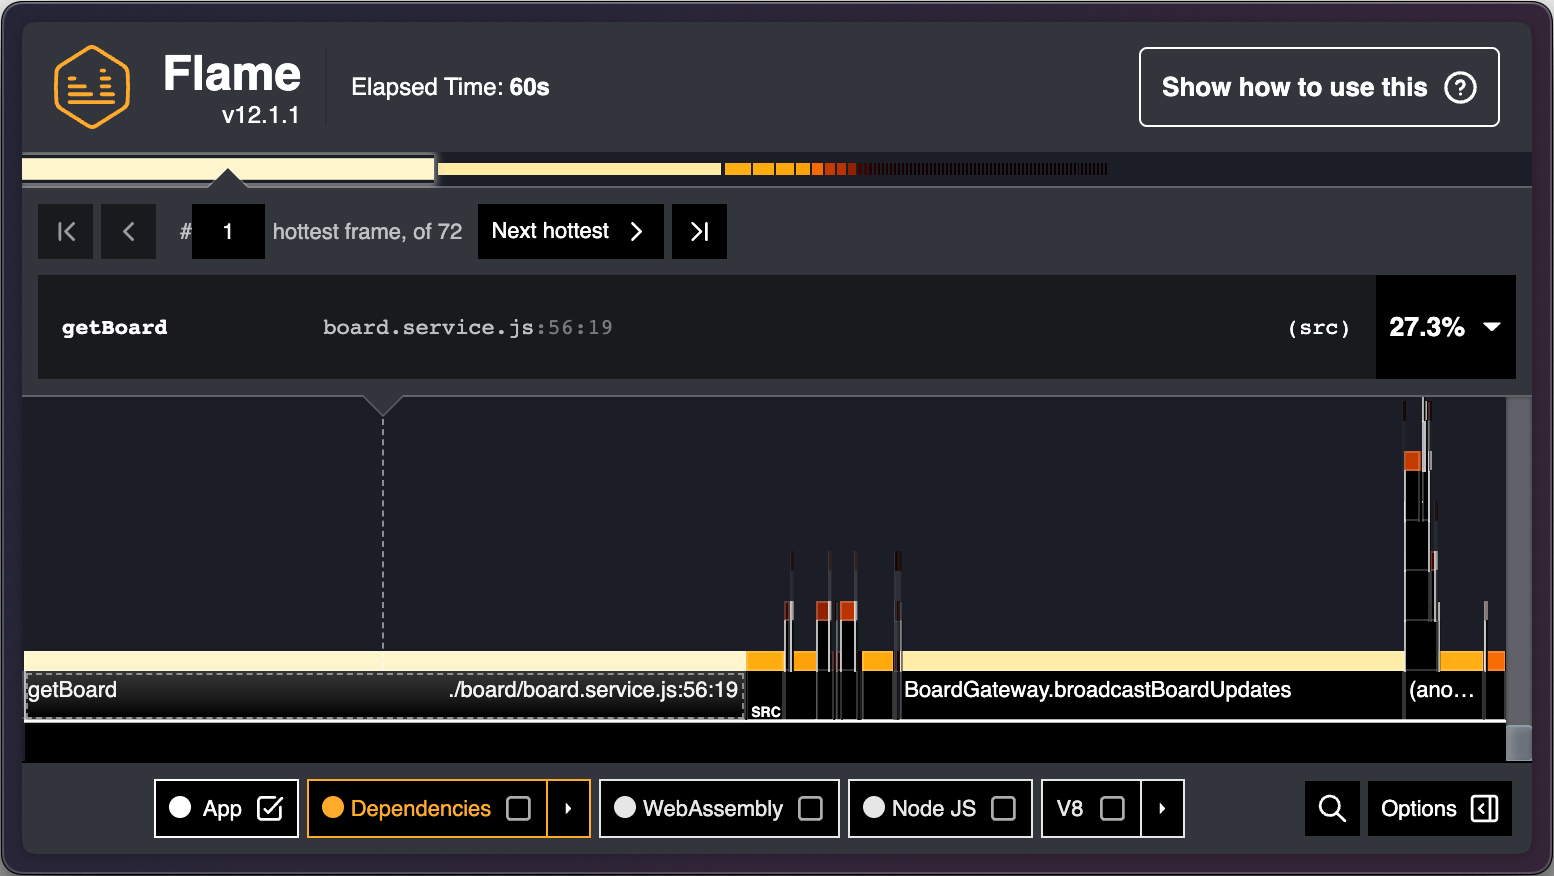
\includegraphics[width=1\textwidth]{./assets/figures/flame/flame3-filtered.png}
  \caption{Code de l'application filtré par Clinic.js}
  \label{fig:flame3-filtered}
\end{figure}

Étonnamment, la figure \ref{fig:flame3-filtered} montre que la fonction \texttt{getBoard} est maintenant la plus coûteuse à 27.3\%, devant \texttt{broadcastBoardUpdates} à seulement 18.8\%  qui était la fonction la plus coûteuse dans les tests précédents. Il est nécessaire de se concentrer sur cette fonction afin de trouver de potentielles optimisations. Tout d'abord, le code de cette fonction est présenté dans le listing \ref{listing:getBoard}.

\begin{listing}[H]
  \begin{minted}[breaklines, linenos]{ts}
  async getBoard() {
    const bitfield = await this.redisClient.get(BOARD_KEY);
    const buffer = Buffer.from(bitfield, UTF8);
    return Array.from(buffer);
  }
\end{minted}
  \caption{Méthode \texttt{getBoard} initiale}
  \label{listing:getBoard}
\end{listing}

Cette méthode se contente de récupérer le Bitfield dans Redis contenant les couleurs de la toile. Ces valeurs se trouvent sous la forme d'une chaîne de caractères qu'il faut ensuite convertir en tableau JavaScript.

\begin{figure}[H]
  \centering
  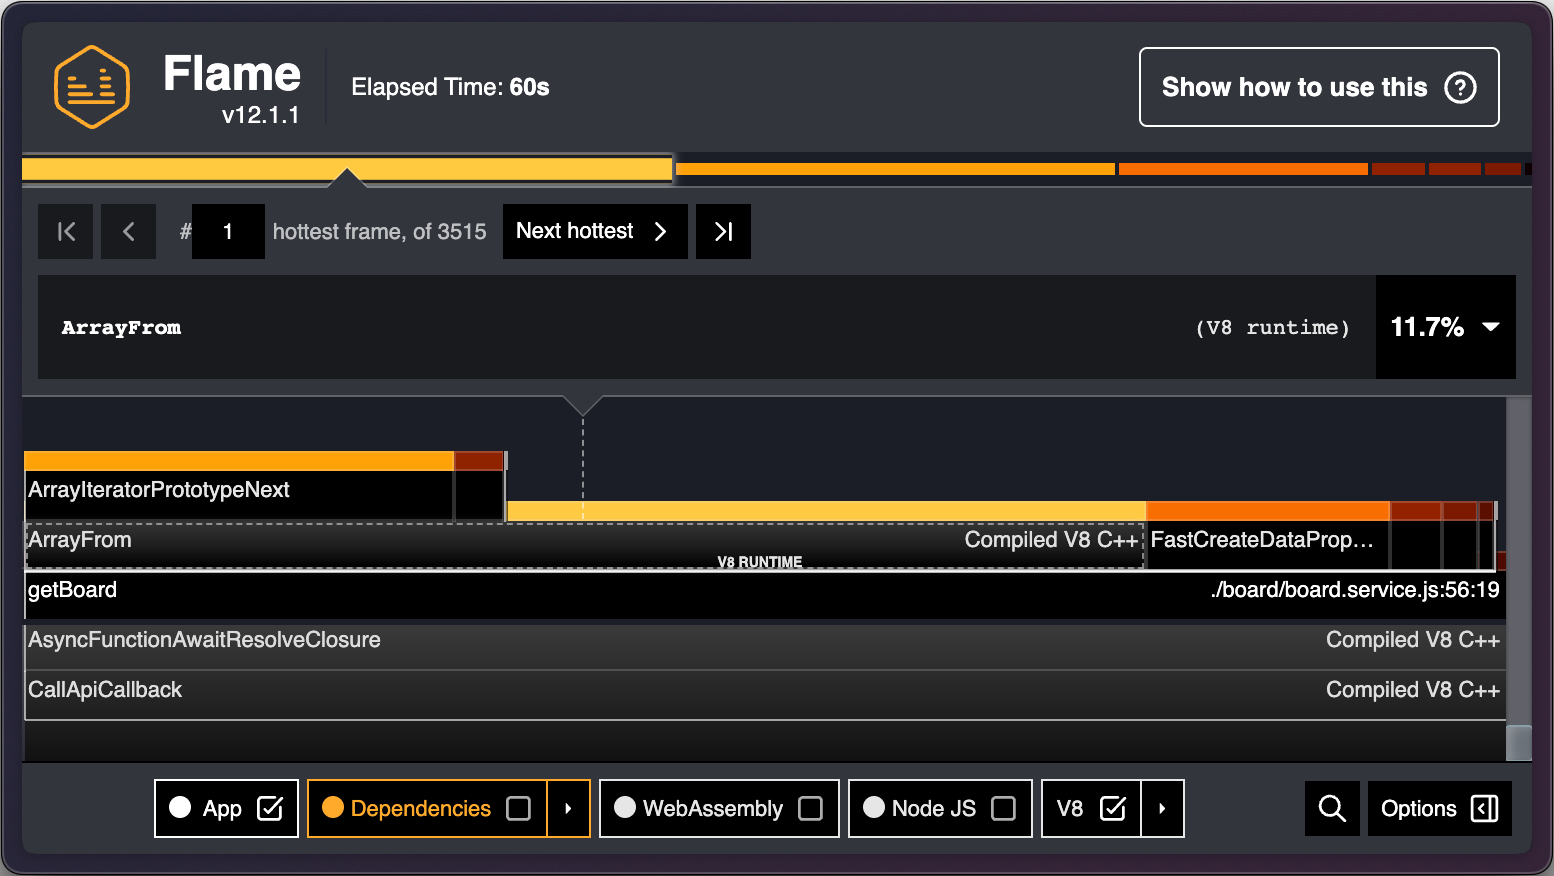
\includegraphics[width=1\textwidth]{./assets/figures/flame/flame3-getBoard.png}
  \caption{Zoom sur la fonction \texttt{getBoard} du rapport Clinic.js}
  \label{fig:flame3-getBoard}
\end{figure}

En mettant l'accent sur cette fonction \texttt{getBoard} dans la figure \ref{fig:flame3-getBoard}, il est possible de voir que la majorité du temps se passe dans la création du tableau JavaScript à l'aide de la fonction \texttt{Array.from} vue précédemment. Il semble donc être intéressant de mettre en cache, dans la mémoire de l'application, le tableau des couleurs de la toile.

\subsubsection{Version optimisée}

\begin{listing}[H]
  \inputminted[highlightlines={4,10,11},linenos]{ts}{assets/figures/opti-storage-1.ts}
  \caption{Optimisation du stockage de la toile - stockage en mémoire}
  \label{listing:opti-storage-1}
\end{listing}

Le tableau des couleurs de la toile, appelé \texttt{board}, est maintenant stocké en mémoire dans l'application comme attribut de la classe \texttt{BoardGateway} comme le montre le listing \ref{listing:opti-storage-1}. Il est récupéré dans le Bitfield Redis au lancement de l'application dans la méthode \texttt{onModuleInit}. La subtilité réside dans le fait qu'il est nécessaire d'attendre que le BitField soit bien initialisé par le \texttt{BoardService} avant de le récupérer. Pour ce faire, la méthode \texttt{setupBoard} du service est appelée avant la récupération du tableau.

\begin{listing}[H]
  \inputminted[highlightlines={9,21},linenos]{ts}{assets/figures/opti-storage-2.ts}
  \caption{Optimisation du stockage de la toile - accès et mise à jour du cache}
  \label{listing:opti-storage-2}
\end{listing}

Par la suite, le tableau en mémoire, \texttt{board}, est envoyé aux utilisateurs se connectant à l'application dans la méthode \texttt{join} afin de pouvoir être affiché. Pour que le tableau soit toujours à jour, son contenu est actualisé en même temps que le Bitfield Redis dans la méthode \texttt{adPixel} lorsqu'un utilisateur pose un nouveau pixel sur la toile.

Il est maintenant possible de relancer les tests de montée en charge pour s'assurer que les performances sont meilleures.

\begin{table}[H]
  \centering
  \begin{tabular}{|l|l|l|l|}
    \hline
    \textbf{Version}  & \textbf{Temps d'exécution} & \textbf{Utilisateurs virtuels} & \textbf{Pixels dessinés} \\ \hline
    64x64 initiale    & 29299.209 ms               & 1342                           & 3088                     \\ \hline
    64x64 optimisée   & 29318.824 ms               & 1347.5                         & 3093                     \\ \Xhline{4\arrayrulewidth}
    256x256 initiale  & 25149.732 ms               & 909                            & 2108                     \\ \hline
    256x256 optimisée & 29243.296 ms               & 1249.5                         & 2921                     \\ \hline
  \end{tabular}
  \caption{Médiane des résultats de 10 tests en changeant la taille de la toile avec la version optimisée}
  \label{table:canvas-size-results-optimized}
\end{table}

Comme le montre la table \ref{table:canvas-size-results-optimized}, les performances entre les deux versions sont quasiment équivalentes lorsque la taille de la toile est de 64x64 pixels. Ce résultat était attendu car les soucis de performances apparaissaient avec une taille plus élevée. Pour la toile de 256x256 pixels, soit 16 fois plus grande, les performances sont bien meilleures avec la nouvelle version optimisée. Ils sont environ 37\% plus rapides que la version précédente et seulement 7\% plus lents que les résultats avec la petite toile de 64x64. Les conclusions de cette optimisation sont donc positives et celle-ci est conservée.

Il aurait également pu être possible d'envoyer directement la chaîne de caractères du Bitfield Redis aux utilisateurs et de laisser le client la convertir en tableau. Cependant, cela aurait demandé au frontend de connaître l'encodage utilisé du côté du backend, ce qui impacte l'évolutivité de la solution.

\subsection{Autres optimisations}

La documentation de Socket.IO~\cite{socket-io-performance-tuning} explique diverses techniques afin d'optimiser les performances de son application. Celles-ci sont regroupées en deux catégories: les optimisations au niveau WebSocket et les optimisations au niveau du système d'exploitation.

\subsubsection{Optimisations au niveau WebSocket}

Concernant les optimisations au niveau WebSocket, il s'agit en réalité pour la plupart d'options déjà testées. Comme par exemple utiliser un parseur customisé lors de l'envoi de données binaires. Socket.IO propose également d'utiliser une autre implémentation WebSocket du côté du serveur appelée \texttt{eiows}. Cependant, ce module n'est pas très utilisé ni maintenu et il n'est pas disponible en TypeScript ni sur Windows. Il n'a donc pas été testé. Socket.IO propose également des modules permettant d'accélérer certaines opérations en utilisant des implémentations natives en C++. Les modules \texttt{bufferutil} et \texttt{utf-8-validate} ont donc été installés mais les gains de performance n'étaient pas véritablement perceptibles. Ils ont quand même été gardés car il s'agit de dépendances optionnelles qui permettent de mieux respecter la spécification WebSocket. Ces dépendances sont utilisées uniquement lorsqu'elles sont disponibles dans l'environnement de l'application.

\subsubsection{Optimisations au niveau du système d'exploitation}

La documentation de Socket.IO explique qu'il existe deux configurations au niveau du système d'exploitation Linux pour accepter un nombre important de connexions en simultané:

\begin{enumerate}
  \item Le nombre maximal de fichiers ouverts en simultané
  \item Le nombre de ports disponibles
\end{enumerate}

Le premier point était initialement limité à 1024, il a donc été passé à plus d'un million comme la documentation le propose. Concernant le nombre de ports, la configuration initiale permettait d'avoir environ 28'000 connexions simultanées. Ce qui est bien au-dessus des besoins du projet. La configuration n'a donc pas été modifiée.

\subsection{Résultats finaux}

Les résultats finaux sont très satisfaisants en ayant en tête les besoins et le public cible de l'application. Toutes les personnes présentes au festival pourront utiliser l'application en simultané sans problème majeur.

Pour rappel, les optimisations finalement réalisées sont les suivantes:

\begin{itemize}
  \item Optimisation du broadcast des pixels avec un intervalle de temps;
  \item Utilisation d'un format sous forme de chaîne de caractères plus léger que le JSON pour envoyer les pixels;
  \item Mise en cache du Bitfield Redis dans la mémoire de l'application;
  \item Installation de dépendances optionnelles pour Socket.IO permettant d'accélérer certaines opérations;
  \item Optimisation de la configuration du système d'exploitation Linux (nombre maximal de fichiers ouverts en simultané).
\end{itemize}

Avec cette version finale optimisée, les résultats sont les suivants pour une toile de 64x64 pixels:

\begin{itemize}
  \item \textbf{Temps d'exécution} (avant d'arriver au seuil des 1.2s de latence): 29291.747 ms
  \item \textbf{Utilisateurs virtuels}: 1341.5
  \item \textbf{Pixels dessinés}: 3087
\end{itemize}

A noter qu'il est tout à fait possible d'augmenter le délai entre deux rafraîchissements afin d'améliorer encore les performances dans des moments critiques. Comme expliqué précédemment, il suffit de modifier la variable d'environnement et de relancer le backend de l'application pour que le changement opère. La valeur des \textbf{100 ms} actuellement utilisée est un bon compromis entre performance et fluidité de l'application. En ajustant la valeur à \textbf{400 ms} par exemple, ce qui reste un délai acceptable pour l'utilisateur, l'application peut supporter jusqu'à \textbf{1737 utilisateurs virtuels} et \textbf{4047 pixels dessinés}.

Il est donc nécessaire de trouver un bon équilibre entre les deux valeurs suivantes afin d'obtenir les performances désirées:

\begin{itemize}
  \item La taille de la toile;
  \item Le délai entre deux rafraîchissements.
\end{itemize}

Heureusement, grâce à toute la mise en place réalisée pour les tests de montée en charge, il est maintenant aisé et rapide de tester différentes configurations et de trouver le bon compromis pour la situation donnée.

\subsubsection{Tests plus réalistes}

Pour conclure, il aurait été intéressant de pouvoir tester les différentes versions avec des tests de montée en charge qui simulent mieux des utilisateurs en utilisant des navigateurs headless (sans interface graphique). En effet, cela aurait permis d'avoir une vision plus réaliste des temps de communication et pas uniquement du point de vue du backend. Malheureusement, les problèmes de ces tests avec navigateurs sont les suivants:

\begin{itemize}
  \item Il est difficile de créer une charge réaliste, un ordinateur, même puissant, ne pourra pas lancer plus de quelques dizaines, voire centaines de navigateurs en simultané
  \item La version de k6 permettant d'utiliser un navigateur headless~\cite{k6-browser} est vraiment expérimentale et peu stable. Il n'a d'ailleurs pas été possible de la faire fonctionner.
\end{itemize}

% FAIT / testé:
% - tentative de ImageData
% - pour frontend: rien fait
